\documentclass{article}
\usepackage[spanish]{babel}
\usepackage[utf8]{inputenc}
\usepackage{tikz}
\usepackage{johd}

\title{Tema 2. Protocolo HTTP}

\author{José Antonio Fajardo Naranjo \\
	\small
	\tt{fajardonaranjoja@gmail.com} \\
	\date{}
}

\begin{document}
	\maketitle
	\begin{abstract} 
		\noindent Estos apuntes pertenecen al tema 2 de la asignatura Desarrollo Web en entorno servidor impartida en el 2ndo curso de FPGS de Desarrollo de aplicaciones web en el IES Martín Rivero durante el curso 2023/2024.
	\end{abstract}
	\newpage{\ }
	\tableofcontents
	\newpage{\ }
	\thispagestyle{empty}
	
	


	\section{Introducción}
	
	\paragraph{}El protocolo HTTP busca la simpleza y la eficacia para el intercambio de documentos. Aunque su uso principal es el intercambio de los documentos de hipertexto se puede usar para transferir otro tipo de elementos.
	
	\subsection{Funcionamiento}
	
	\paragraph{}El principio en el que se basa este protocolo es el tándem pregunta/respuesta. El cliente genera una pregunta con la forma de una petición HTTP que contiene, al menos, los datos que permiten identificar el recurso que le ha sido solicitado por el cliente. Esta petición no es más que un bloque de texto que viaja del cliente al servidor. Se compone de dos partes separadas por una línea en blanco (retorno de carro o salto de línea). La primera parte es la cabecera de la petición HTTP, que es obligatoria, mientras que la segunda es el cuerpo, que es opcional, dependiendo su aparición del tipo de petición HTTP. La línea en blanco ha de aparecer siempre, siendo completamente \textbf{obligatoria}. La respuesta mantiene el mismo formato de las peticiones.
	
	\paragraph{}Una respuesta HTTP sólo existe si se ha enviado previamente una petición HTTP al servidor, no tomando este último la iniciativa de enviar datos que no han sido solicitados por el cliente (con la tecnología de los \textbf{WebSockets} esto no es necesario, los servidores actualizan en tiempo real sin necesidad de petición).
	
	\paragraph{}El protocolo TCP se utiliza para el transporte de los bloques de texto de petición y respuesta HTTP. Por defecto, esta conexión mediante TCP se establece para cada par petición/respuesta. Sin embargo, la versión 1.1 propone una solución para transportar varios pares petición/respuesta con la misma conexión TCP. A continuación, encontramos el ejemplo utilizado en clase de paquete capturado.
	
	\begin{figure}[H]
		\centering
		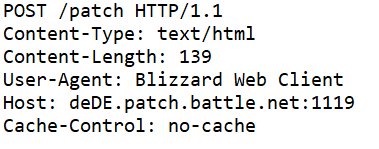
\includegraphics[scale=0.5]{images/peticionhttp.PNG}
		\caption{\label{fig1}Captura de una petición HTTP}
	\end{figure}
	
	\begin{figure}[H]
		\centering
		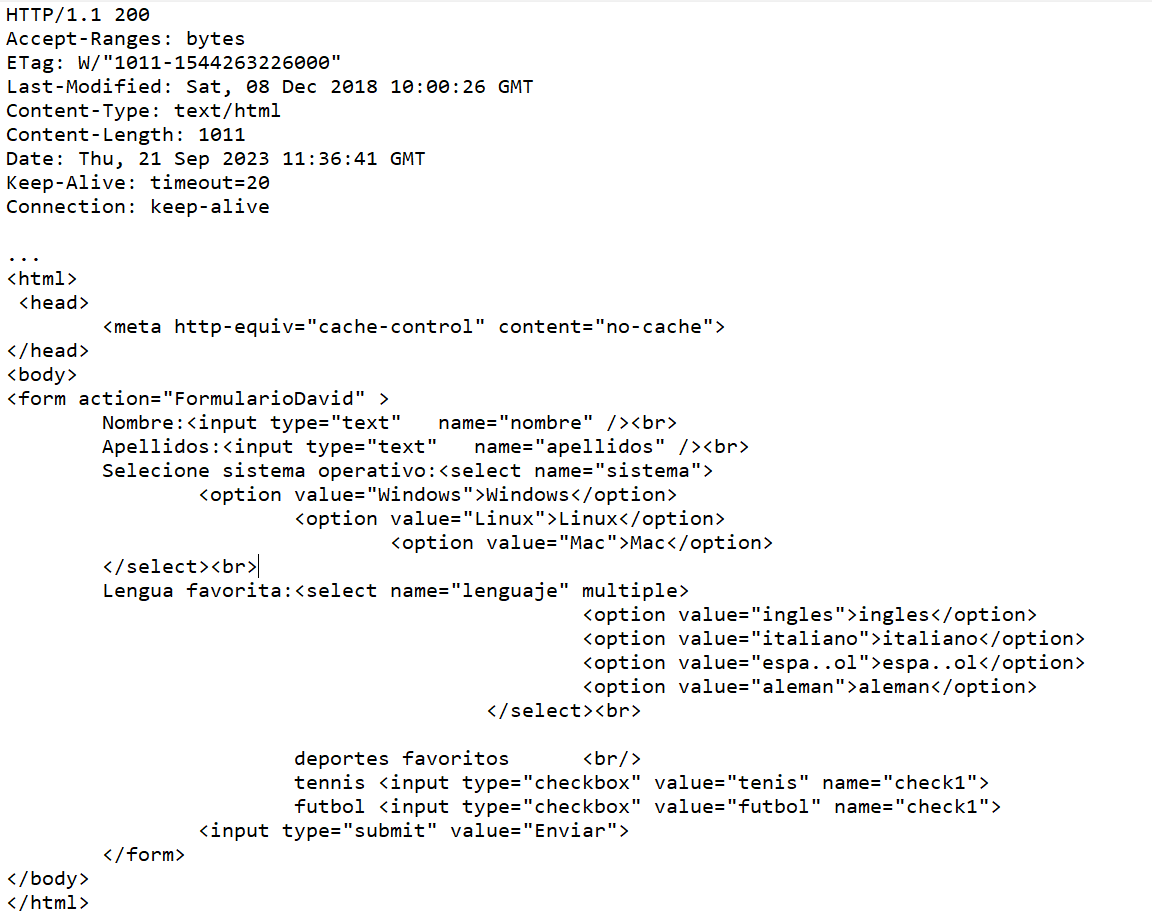
\includegraphics[scale=0.5]{images/respuestahttp.png}
		\caption{\label{fig2}Captura de una respuesta HTTP}
	\end{figure}
	
	\subsection{Las URL}
	
	\paragraph{}Las URL (Uniform Resource Locator) permiten localizar los recursos que se desean recuperar mediante peticiones HTTP. Se componen de una cadena de caracteres de cinco campos. Se ha de seguir el siguiente formato:
	
	\begin{center}
			\texttt{protocolo://identificador del servidor:número de puerto/recurso?parámetros}
	\end{center}
	
	\begin{itemize}
		\item Protocolo: indica el protocolo utilizado para el acceso al recurso. Nosotros usaremos HTTP aunque hay otros como FTP o mailto.
		\item Identificador del servidor: esta parte permite localizar el servidor en la red. Normalmente es el FQDN (Fully Qualified Domain Name), el nombre de dominio del servidor, que no da lugar a ambigüedades. Se tiene que transformar en la dirección IP para que el protocolo TCP pueda establecer una conexión con el servidor, de lo cual se encarga un servidor DNS (Domain Name System). Se puede usar una IP en la URL pero es más sencillo el FQDN.
		\item Número de puerto: este dato es el número de puerto TCP con el que se debe establecer la conexión. Este número funciona para que el protocolo TCP identifique una aplicación particular en una máquina. Este sistema permite el alojamiento de más de una aplicación por servidor. El puerto 80 es el que se asigna por defecto al protocolo HTTP.
		\item Recurso: esta parte de la URL permite determinar el recurso que se desea obtener. Puede estar compuesto por varios elementos separados por el carácter.
		\item Parámetros: son los datos que pasamos cuando la petición HTTP se hace, por ejemplo, sobre un recurso dinámico. Aparecen de la forma nombreDeParam=valorDeParam. Con el carácter \& se pueden separar estos parámetros.
	\end{itemize}
	
	\paragraph{}A continuación se muestran equivalencias entre los caracteres y su valor en ASCII, ya que algunos caracteres tienen una función en las URL:
	
	\begin{table}[H]
		\centering
		\begin{tabular}{|l|l|}
			\hline
			\multicolumn{1}{|c|}{\textbf{Carácter}} & \multicolumn{1}{c|}{\textbf{Codificación}} \\ \hline
			Espacio                                 & \%20 o a veces +                           \\ \hline
			"                                       & \%22                                       \\ \hline
			\%                                      & \%25                                       \\ \hline
			\&                                      & \%26                                       \\ \hline
			+                                       & \%2B                                       \\ \hline
			.                                       & \%2E                                       \\ \hline
			/                                       & \%2F                                       \\ \hline
			?                                       & \%3F                                       \\ \hline
			'                                       & \%60                                       \\ \hline
		\end{tabular}
	\end{table}
	
	\section{Las peticiones HTTP}
	
	\paragraph{}Las peticiones HTTP comienzan el diálogo entre un navegador (cliente) y un servidor Web. El navegador, por norma general, construye la petición HTTP en función de los datos contenidos en una página HTML. Todas las cabeceras de una petición comienzan por una línea con el mismo formato, contiene el tipo de la petición HTTP seguido del identificador del recurso solicitado y finaliza con la versión del protocolo HTTP (HTTP/1.1).
	
	\subsection{Los distintos tipos de petición}
	
	\paragraph{}La versión 1.0 del protocolo HTTP disponía de 3 tipos de petición HTTP:
	
	 \begin{itemize}
	 	\item GET: permite obtener un recurso disponible en el servidor. Es el tipo que se genera por defecto. No tiene ningún tipo de dato en el cuerpo de la petición y si necesita enviar parámetros al servidor se añaden a continuación de la URL.
	 	\item POST: se destina al envío al servidor de datos recopilados en formularios HTML. Presenta ventajas con respecto al método GET.
	 		\subitem No hay límite teórico de cantidad de información que se envía, porque se inserta en el cuerpo de la petición en lugar de en la cabecera.
	 		\subitem No se ven los datos en la barra de dirección del navegador, por lo cual existe más privacidad.
	 	\item HEAD: funciona como la petición GET, salvo porque el servidor no devuelve nada en el cuerpo de la respuesta HTTP. Los navegadores lo utilizan para la gestión del almacenamiento en caché de datos.
	 \end{itemize}
	
	\paragraph{}La versión 1.1 de protocolo HTTP añade nuevos tipos de petición.
	
	\begin{itemize}
		\item La petición PUT permite enviar un recurso al servidor para que éste lo guarde de forma permanente.
		\item La petición DELETE permite solicitar la eliminación de un recurso determinado.
		\item La petición TRACE permite solicitar al servidor la devolución en el cuerpo de la respuesta HTTP de una copia de la petición HTTP que acaba de recibir.
		\item La petición OPTIONS permite obtener datos sobre las opciones que se pueden utilizar para obtener un recurso.
	\end{itemize}
	
	\subsection{Las cabeceras de petición}
	
	\paragraph{}El cliente (navegador) añade las cabeceras de petición en el momento en que construye la petición HTTP. Cada tipo de navegador construye y ordena la cabecera de la petición HTTP de manera diferente. La función de estas es la de proporcionar al servidor información adicional acerca de la petición. Hay algunas que se consideran estándar y aparecen en todas las peticiones. Entre las más comunes se destacan:
	
	\begin{itemize}
		\item \texttt{Accept}: esta cabecera permite indicar al servidor qué tipos de datos se aceptan como respuesta. El formato en el que se tienen que indicar este tipo de datos es el MIME (Multipurpose Internet Main Extensions). Si el navegador no tiene ninguna preferencia, puede añadir la cabecera siguiente:
		\begin{center}
			\texttt{Accept: */*}
		\end{center}
		\item \texttt{Accept-Charset}: esta cabecera indica las preferencias respecto al juego de caracteres que puede usar el servidor para construir la respuesta HTTP. Ejemplo:
		\begin{center}
			\texttt{Accept-Charset: ISO-8559-1,utf-8}
		\end{center}
		\item \texttt{Accept-Encoding}: esta cabecera indica al servidor en qué lengua prefiere obtener el recurso solicitado. Ejemplo:
		\begin{center}
			\texttt{Accept-Language: es,en}
		\end{center}
		\item \texttt{Connection}: esta cabecera es de la versión 1.1 de HTTP. Determina cómo se comportarán las conexiones TCP utilizadas para la petición y la respuesta. Si el navegador desea mantener la conexión abierta puede añadir valor keep-alive para la cabecera. Por el contrario, con el valor close la conexión se cierra. Ejemplo:
		\begin{center}
			\texttt{Connection: keep-alive}
		\end{center}
		\item \texttt{Host}: esta cabecera de la versión 1.1 del protocolo HTTP especifica el FQDN (Fully Qualified Domain Name) y el número del puerto del servidor que aloja el recurso solicitado. Este nombre puede corresponder a un servidor físico o a uno virtual. Siempre es necesario que pueda transformarse en una dirección IP para que el protocolo TCP pueda transportar la petición HTTP. En caso de que se usen servidores virtuales hay varios FQDN con la misma dirección IP. La referencia hacia el servidor virtual adecuado se realiza con esta cabecera. 
		\begin{center}
			\texttt{Host: www.eni-ecole.fr}
		\end{center}
		\item \texttt{Referer}: esta cabecera contiene la URL del documento a partir del cual la petición HTTP ha sido generada. Se informa cuando una petición HTTP se construye después de la activación de un enlace de hipertexto o de la validación de un formulario. Ejemplo:
		\begin{center}
			\texttt{GET /index.php HTTP/1.1\\
			Referer: http://www.eni-ecole.fr/}
		\end{center}
		\item User-Agent: esta cabecera permite identificar el tipo de navegador en el origen de la petición, pudiendo utilizarse para realizar estadísticas o permitir al servidor optimizar el código enviado en función del tipo de navegador (especie de firma del navegador). Ejemplo:
		\begin{center}
			\texttt{poner ejemplo}
		\end{center}
	\end{itemize}
	
\end{document}